\documentclass{standalone}
\usepackage{tikz}
\usetikzlibrary{patterns, positioning}


\begin{document}
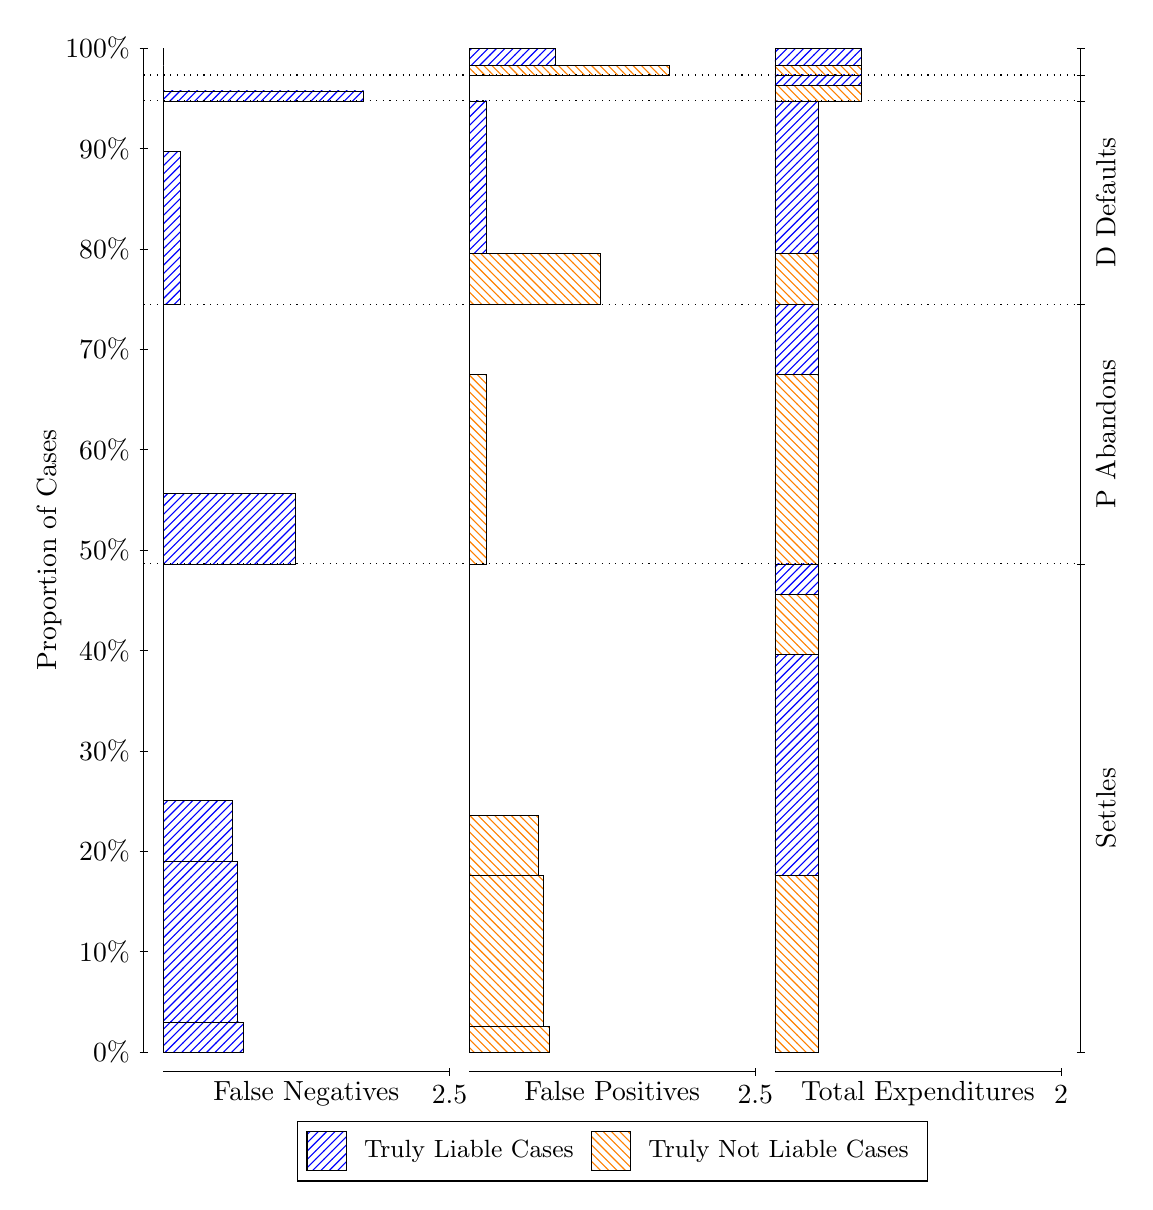
\begin{tikzpicture}
\draw[black, very thin] (1.5,1.75) -- (1.5,14.5);
\node[rotate=90, text=black, anchor=center] at (0.3, 8.125) {Proportion of Cases};
\draw[black, very thin] (1.45,1.75) -- (1.55,1.75);
\node[text=black, anchor=east] at (1.45, 1.75) {0\%};
\draw[black, very thin] (1.45,3.025) -- (1.55,3.025);
\node[text=black, anchor=east] at (1.45, 3.025) {10\%};
\draw[black, very thin] (1.45,4.3) -- (1.55,4.3);
\node[text=black, anchor=east] at (1.45, 4.3) {20\%};
\draw[black, very thin] (1.45,5.575) -- (1.55,5.575);
\node[text=black, anchor=east] at (1.45, 5.575) {30\%};
\draw[black, very thin] (1.45,6.85) -- (1.55,6.85);
\node[text=black, anchor=east] at (1.45, 6.85) {40\%};
\draw[black, very thin] (1.45,8.125) -- (1.55,8.125);
\node[text=black, anchor=east] at (1.45, 8.125) {50\%};
\draw[black, very thin] (1.45,9.4) -- (1.55,9.4);
\node[text=black, anchor=east] at (1.45, 9.4) {60\%};
\draw[black, very thin] (1.45,10.675) -- (1.55,10.675);
\node[text=black, anchor=east] at (1.45, 10.675) {70\%};
\draw[black, very thin] (1.45,11.95) -- (1.55,11.95);
\node[text=black, anchor=east] at (1.45, 11.95) {80\%};
\draw[black, very thin] (1.45,13.225) -- (1.55,13.225);
\node[text=black, anchor=east] at (1.45, 13.225) {90\%};
\draw[black, very thin] (1.45,14.5) -- (1.55,14.5);
\node[text=black, anchor=east] at (1.45, 14.5) {100\%};

\draw[black, very thin] (13.4,1.75) -- (13.4,14.5);
\draw[black, very thin] (13.35,1.75) -- (13.45,1.75);
\node[anchor=west] at (13.35, 1.75) {};
\draw[black, very thin] (13.35,7.9482) -- (13.45,7.9482);
\node[anchor=west] at (13.35, 7.9482) {};
\draw[black, very thin] (13.35,11.246) -- (13.45,11.246);
\node[anchor=west] at (13.35, 11.246) {};
\draw[black, very thin] (13.35,13.829) -- (13.45,13.829);
\node[anchor=west] at (13.35, 13.829) {};
\draw[black, very thin] (13.35,14.158) -- (13.45,14.158);
\node[anchor=west] at (13.35, 14.158) {};
\draw[black, very thin] (13.35,14.5) -- (13.45,14.5);
\node[anchor=west] at (13.35, 14.5) {};

\draw[black, very thin, pattern color=blue, pattern=north east lines] (1.75,1.75) rectangle (2.7673,2.1333);
\draw[black, very thin, pattern color=blue, pattern=north east lines] (1.75,2.1333) rectangle (2.6947,4.1703);
\draw[black, very thin, pattern color=blue, pattern=north east lines] (1.75,4.1703) rectangle (2.622,4.9455);
\draw[black, very thin, pattern color=orange, pattern=north west lines] (1.75,4.9455) rectangle (1.75,7.9482);
\draw[black, very thin, pattern color=blue, pattern=north east lines] (1.75,7.9482) rectangle (3.4213,8.8421);
\draw[black, very thin, pattern color=orange, pattern=north west lines] (1.75,8.8421) rectangle (1.75,11.246);
\draw[black, very thin, pattern color=blue, pattern=north east lines] (1.75,11.246) rectangle (1.968,13.184);
\draw[black, very thin, pattern color=orange, pattern=north west lines] (1.75,13.184) rectangle (1.75,13.829);
\draw[black, very thin, pattern color=blue, pattern=north east lines] (1.75,13.829) rectangle (4.2933,13.957);
\draw[black, very thin, pattern color=orange, pattern=north west lines] (1.75,13.957) rectangle (1.75,14.158);
\draw[black, very thin, pattern color=orange, pattern=north west lines] (1.75,14.158) rectangle (1.75,14.281);
\draw[black, very thin, pattern color=blue, pattern=north east lines] (1.75,14.281) rectangle (1.75,14.5);
\draw[black, very thin, pattern color=orange, pattern=north west lines] (5.6333,1.75) rectangle (6.6507,2.071);
\draw[black, very thin, pattern color=orange, pattern=north west lines] (5.6333,2.071) rectangle (6.578,3.9919);
\draw[black, very thin, pattern color=orange, pattern=north west lines] (5.6333,3.9919) rectangle (6.5053,4.7527);
\draw[black, very thin, pattern color=blue, pattern=north east lines] (5.6333,4.7527) rectangle (5.6333,7.9482);
\draw[black, very thin, pattern color=orange, pattern=north west lines] (5.6333,7.9482) rectangle (5.8513,10.352);
\draw[black, very thin, pattern color=blue, pattern=north east lines] (5.6333,10.352) rectangle (5.6333,11.246);
\draw[black, very thin, pattern color=orange, pattern=north west lines] (5.6333,11.246) rectangle (7.3047,11.891);
\draw[black, very thin, pattern color=blue, pattern=north east lines] (5.6333,11.891) rectangle (5.8513,13.829);
\draw[black, very thin, pattern color=orange, pattern=north west lines] (5.6333,13.829) rectangle (5.6333,14.03);
\draw[black, very thin, pattern color=blue, pattern=north east lines] (5.6333,14.03) rectangle (5.6333,14.158);
\draw[black, very thin, pattern color=orange, pattern=north west lines] (5.6333,14.158) rectangle (8.1767,14.281);
\draw[black, very thin, pattern color=blue, pattern=north east lines] (5.6333,14.281) rectangle (6.7233,14.5);
\draw[black, very thin, pattern color=orange, pattern=north west lines] (9.5167,1.75) rectangle (10.062,3.9919);
\draw[black, very thin, pattern color=blue, pattern=north east lines] (9.5167,3.9919) rectangle (10.062,6.8041);
\draw[black, very thin, pattern color=orange, pattern=north west lines] (9.5167,6.8041) rectangle (10.062,7.5649);
\draw[black, very thin, pattern color=blue, pattern=north east lines] (9.5167,7.5649) rectangle (10.062,7.9482);
\draw[black, very thin, pattern color=orange, pattern=north west lines] (9.5167,7.9482) rectangle (10.062,10.352);
\draw[black, very thin, pattern color=blue, pattern=north east lines] (9.5167,10.352) rectangle (10.062,11.246);
\draw[black, very thin, pattern color=orange, pattern=north west lines] (9.5167,11.246) rectangle (10.062,11.891);
\draw[black, very thin, pattern color=blue, pattern=north east lines] (9.5167,11.891) rectangle (10.062,13.829);
\draw[black, very thin, pattern color=orange, pattern=north west lines] (9.5167,13.829) rectangle (10.607,14.03);
\draw[black, very thin, pattern color=blue, pattern=north east lines] (9.5167,14.03) rectangle (10.607,14.158);
\draw[black, very thin, pattern color=orange, pattern=north west lines] (9.5167,14.158) rectangle (10.607,14.281);
\draw[black, very thin, pattern color=blue, pattern=north east lines] (9.5167,14.281) rectangle (10.607,14.5);
\draw[black, dotted] (1.5,7.9482) -- (13.4,7.9482);
\draw[black, dotted] (1.5,11.246) -- (13.4,11.246);
\draw[black, dotted] (1.5,13.829) -- (13.4,13.829);
\draw[black, dotted] (1.5,14.158) -- (13.4,14.158);
\draw[black, very thin] (1.75,1.5) -- (5.3833,1.5);
\node[text=black, anchor=north] at (3.5667, 1.5) {False Negatives};
\draw[black, very thin] (5.3833,1.45) -- (5.3833,1.55);
\node[text=black, anchor=north] at (5.3833, 1.45) {2.5};

\draw[black, very thin] (5.6333,1.5) -- (9.2667,1.5);
\node[text=black, anchor=north] at (7.45, 1.5) {False Positives};
\draw[black, very thin] (9.2667,1.45) -- (9.2667,1.55);
\node[text=black, anchor=north] at (9.2667, 1.45) {2.5};

\draw[black, very thin] (9.5167,1.5) -- (13.15,1.5);
\node[text=black, anchor=north] at (11.333, 1.5) {Total Expenditures};
\draw[black, very thin] (13.15,1.45) -- (13.15,1.55);
\node[text=black, anchor=north] at (13.15, 1.45) {2};

\node[text=black, centered, rotate=90] at (13.72, 4.8491) {Settles};
\node[text=black, centered, rotate=90] at (13.72, 9.5973) {P Abandons};
\node[text=black, centered, rotate=90] at (13.72, 12.538) {D Defaults};



\draw (7.449999999999999,1.5) node[draw=none] (baseCoordinate) {};
\begin{scope}[align=center]
        \matrix[scale=0.5, draw=black, below=0.5cm of baseCoordinate, nodes={draw}, column sep=0.1cm]{
            \node[rectangle, draw, minimum width=0.5cm, minimum height=0.5cm, pattern color=blue, pattern=north east lines] {}; &
            \node[draw=none, font=\small, text=black] (B) {Truly Liable Cases}; &
            \node[rectangle, draw, minimum width=0.5cm, minimum height=0.5cm, pattern color=orange, pattern=north west lines] {}; &
            \node[draw=none, font=\small, text=black] (B) {Truly Not Liable Cases}; \\
            };
\end{scope}

\end{tikzpicture}
\end{document}